\documentclass[table]{beamer}


\usepackage{array}
\usepackage{arydshln}
\usepackage{latexsym}
\usepackage{multirow}
\usepackage{amsmath}
\usepackage{amsthm}
\usepackage{rotating}
\usepackage{color}
\usepackage{qtree}
\usepackage{graphicx}
\usepackage{caption}
\usepackage{placeins}
\usepackage{tabularx}
\usepackage{fixltx2e}
\usepackage{hyperref}
\usepackage{subcaption}
\captionsetup{compatibility=false}
\usepackage{xcolor}

% \input{Commands}

\begin{document}
%\title{BEER}   
\title{Discriminative Training}
\subtitle{MT Marathon lecture}
\author{Milo\v{s} Stanojevi\'{c}}
%\author{Milo\v{s} Stanojevi\'{c}\inst{1} \and Amir Kamran\inst{1} \and Ond\v{r}ej Bojar\inst{2}}
%\setbeamerfont{institute}{size=\large}
\institute{ILLC, University of Amsterdam}
%\institute[shortinst]{\inst{1} ILLC, University of Amsterdam \and %
%                      \inst{2} MFF \'UFAL, Charles University in Prague}
\date{\today} 


\frame{\titlepage} 

% \frame{\frametitle{Table of contents}\tableofcontents} 


\newcommand{\argmax}[1]{\underset{#1}{\mathrm{argmax}}\ }

\newcommand{\highlight}[1]{%
  \colorbox{red!50}{$\displaystyle#1$}}

\newlength{\overwritelength}
\newlength{\minimumoverwritelength}
\setlength{\minimumoverwritelength}{1cm}
\newcommand{\overwrite}[3][red]{%
  \settowidth{\overwritelength}{$#2$}%
  \ifdim\overwritelength<\minimumoverwritelength%
    \setlength{\overwritelength}{\minimumoverwritelength}\fi%
  \stackrel
    {%
      \begin{minipage}{\overwritelength}%
        \color{#1}\centering\small #3\\%
        \rule{1pt}{9pt}%
      \end{minipage}}
    {\colorbox{#1!50}{\color{black}$\displaystyle#2$}}}



\frame{\frametitle{Going from Generative to Discriminative models}
Start with generative noisy channel model:
\begin{align}
t^* & = \argmax{t \in T(s)} p(t|s) 
\onslide<2->{ = \argmax{t \in T(s)}  \frac{p(s|t)p(t)}{p(s)}}
\onslide<3->{ = \argmax{t \in T(s)}  p(s|t)p(t)  \nonumber \\}
\onslide<4->{& = \argmax{t \in T(s)}  \log p(s|t) + \log p(t)  \nonumber \\}
\onslide<5->{& = \argmax{t \in T(s)}  \begin{bmatrix} 1 & 1 \end{bmatrix} \begin{bmatrix}\log p(s|t) \\ \log p(t)\end{bmatrix} \nonumber \\}
\onslide<6->{& = \highlight{\argmax{t \in T(s)}  \mathbf{\lambda}^T \mathbf{h}(s,t)} \text{\ \ \ \ \ \ end with linear discriminative model} \nonumber}
\end{align}
% \onslide<6->{End with linear discriminative model}
\onslide<7->{
Why would we want to do this?
\onslide<8->{
\begin{itemize}
\item We can add more indicators (features) of good translation
\onslide<9->{\item We can give different weight to different features
\onslide<10->{\item And all this done in a way to directly optimize desired metric}
\end{itemize}
}
}
}
\onslide<11->{
Disadvantage? Losing probabilistic interpretation
}

}


%\frame{\frametitle{Useful features}
	TODO

}



\frame{\frametitle{Optimize for BLEU directly}
\begin{center}
\only<1>{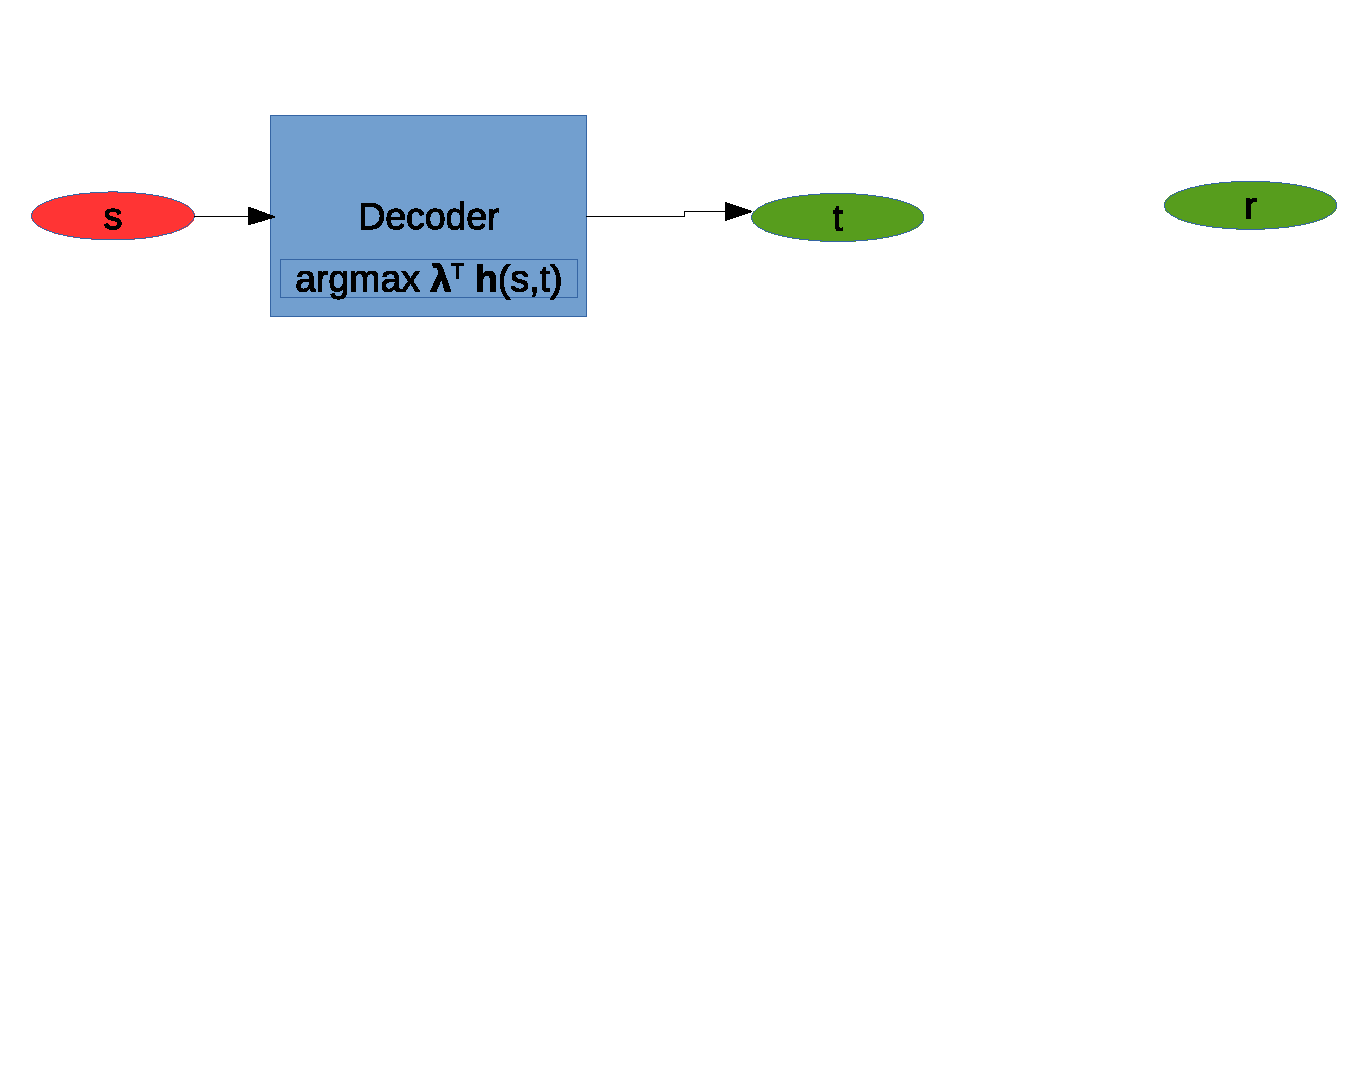
\includegraphics[width=0.70\linewidth]{drawing_discriminative_decoder_tuning1}}
\only<2>{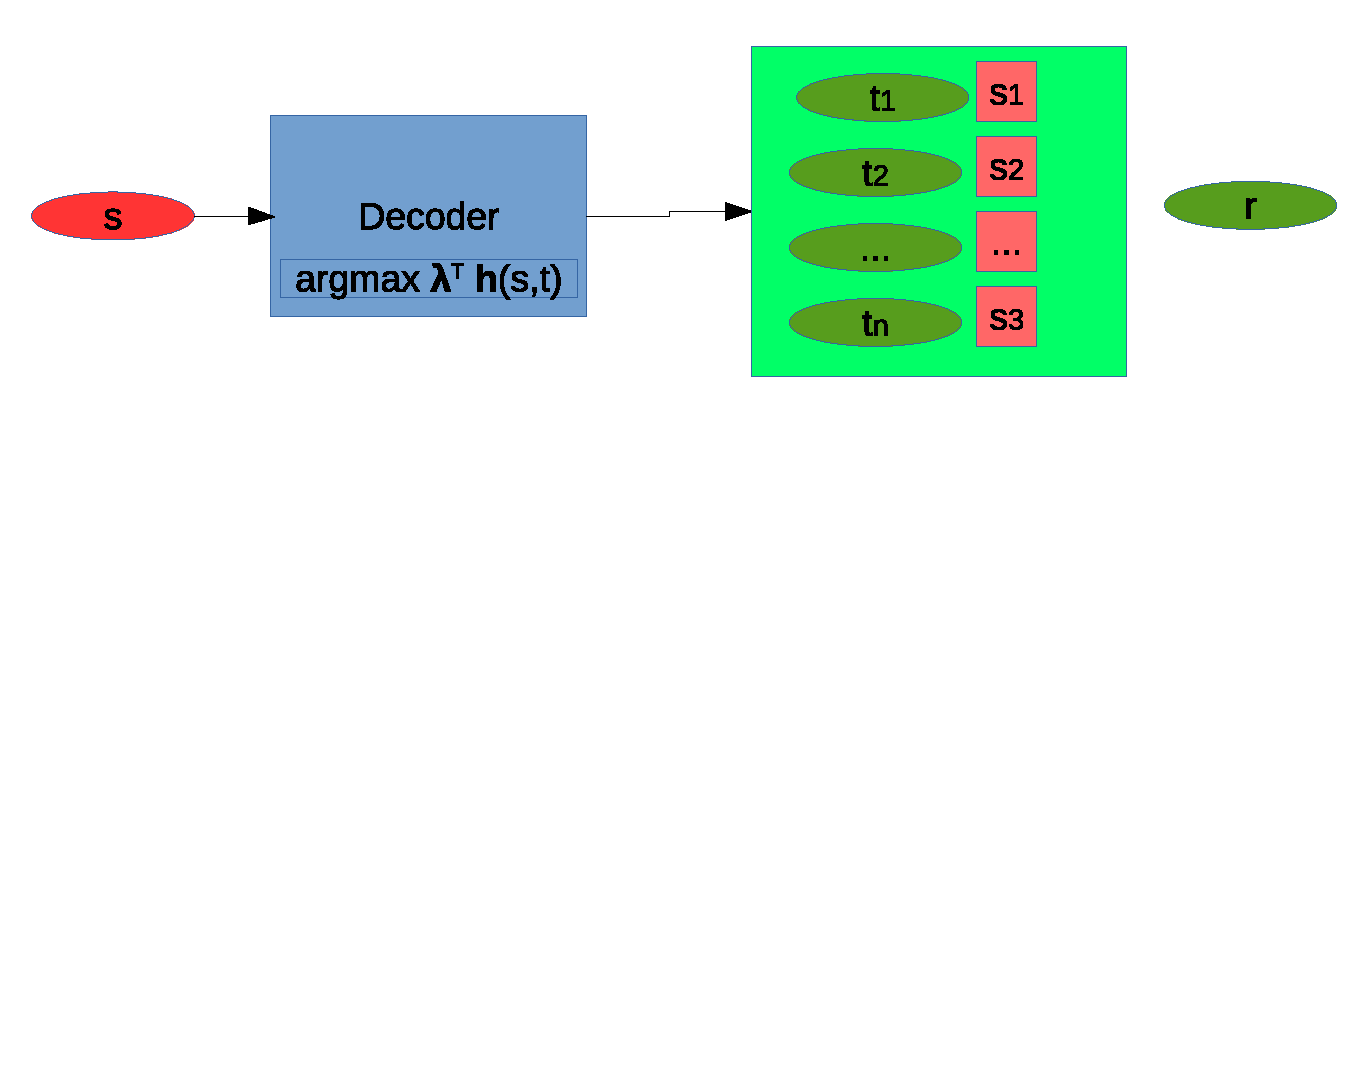
\includegraphics[width=0.70\linewidth]{drawing_discriminative_decoder_tuning2}}
\only<3>{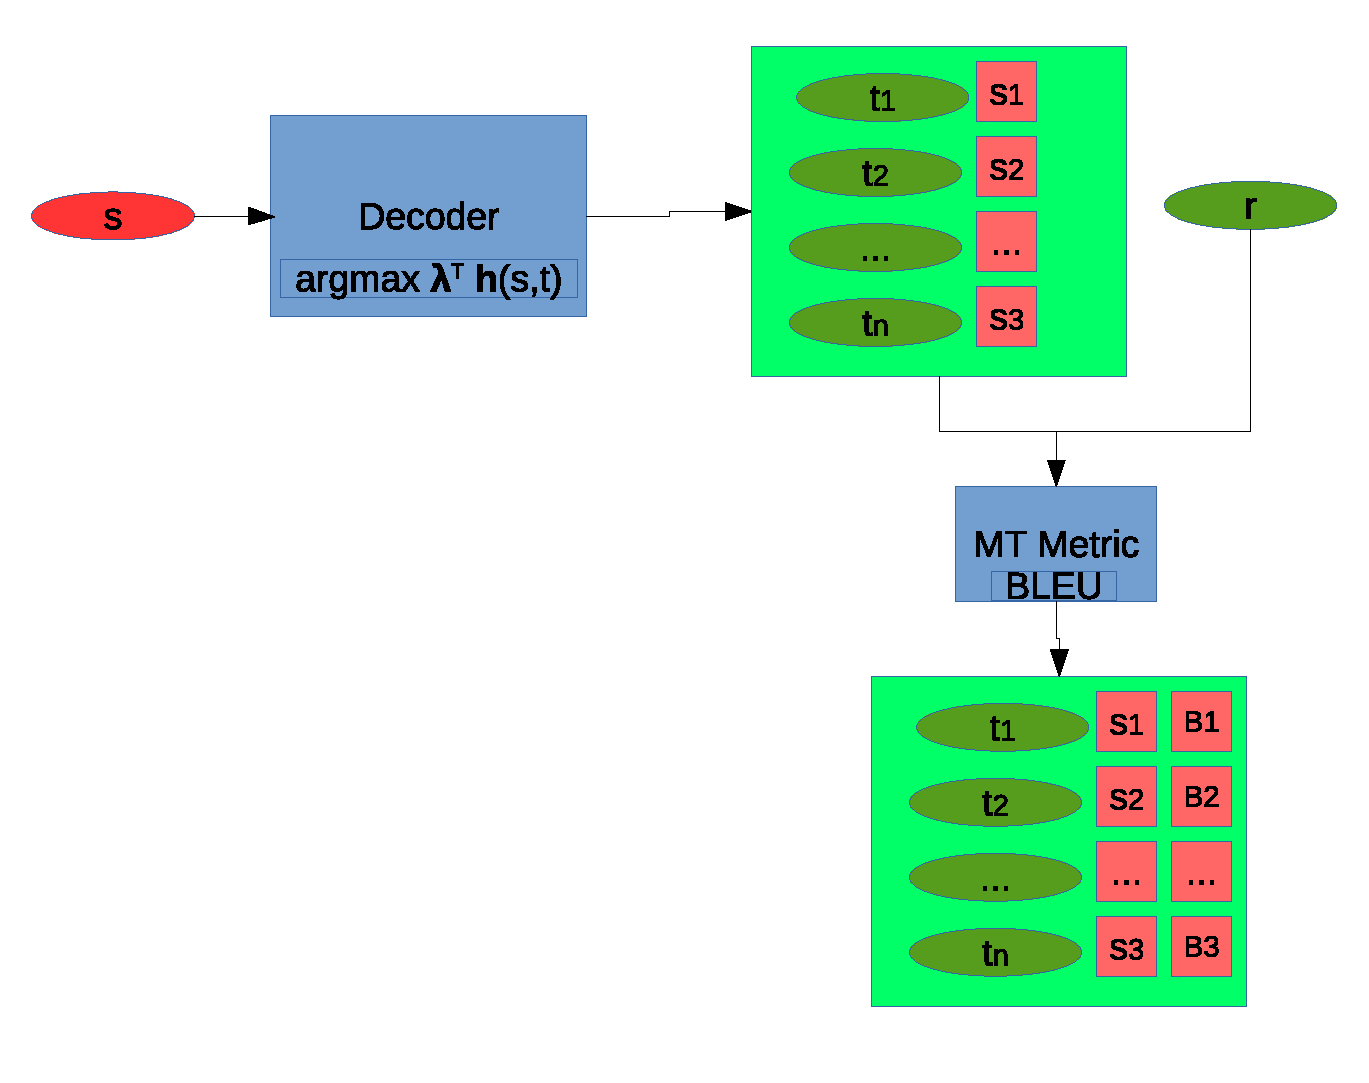
\includegraphics[width=0.70\linewidth]{drawing_discriminative_decoder_tuning3}}
\only<4>{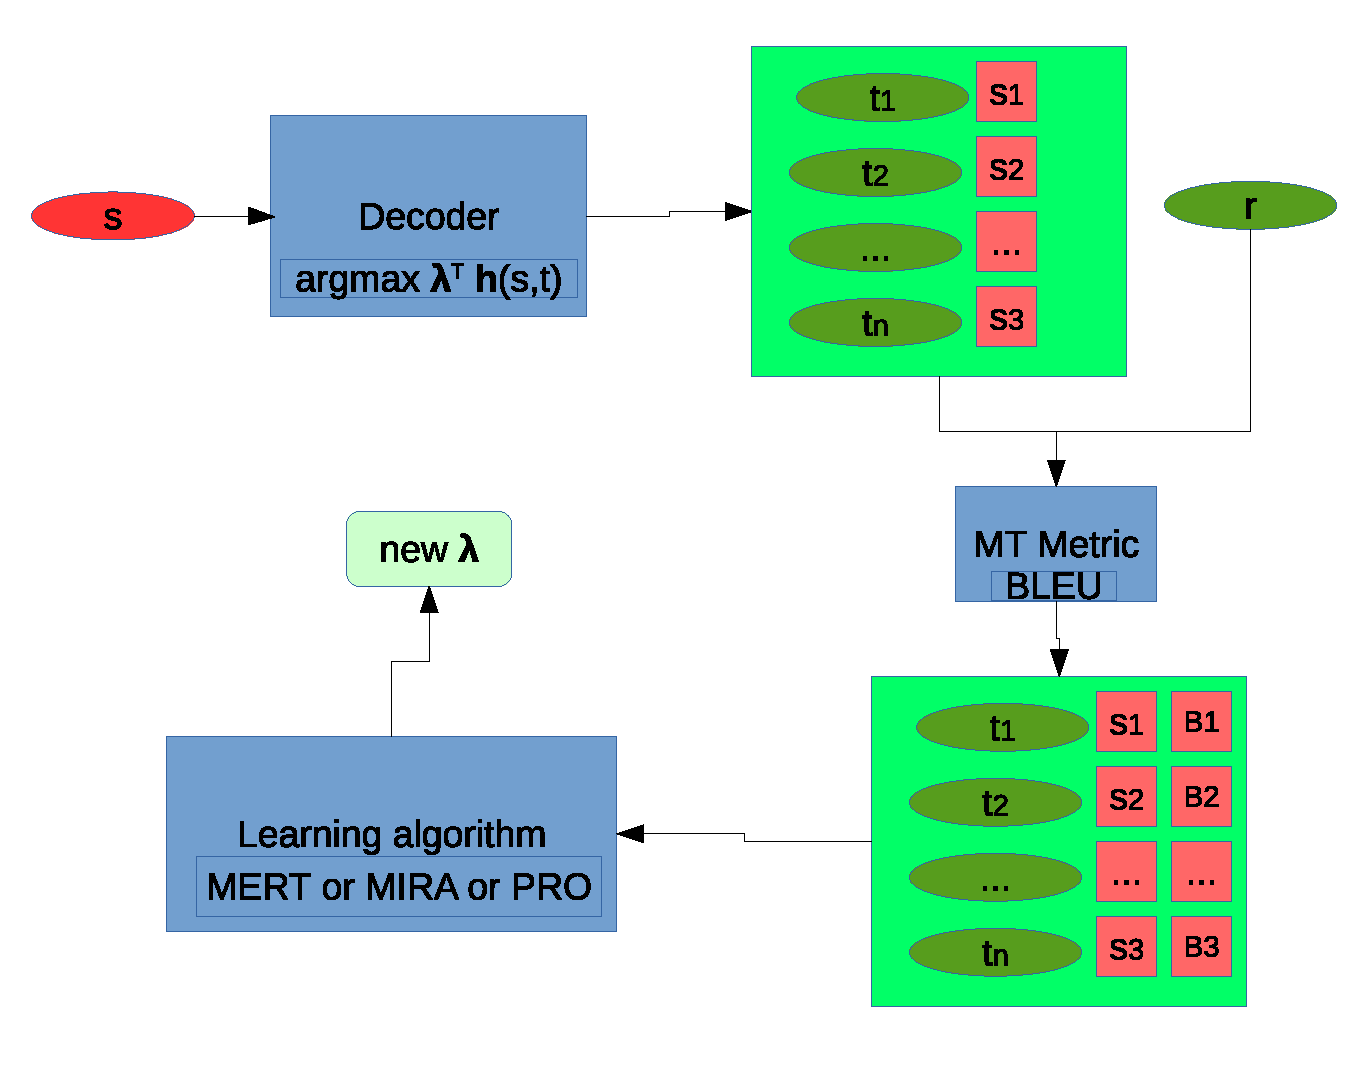
\includegraphics[width=0.70\linewidth]{drawing_discriminative_decoder_tuning4}}
\only<5>{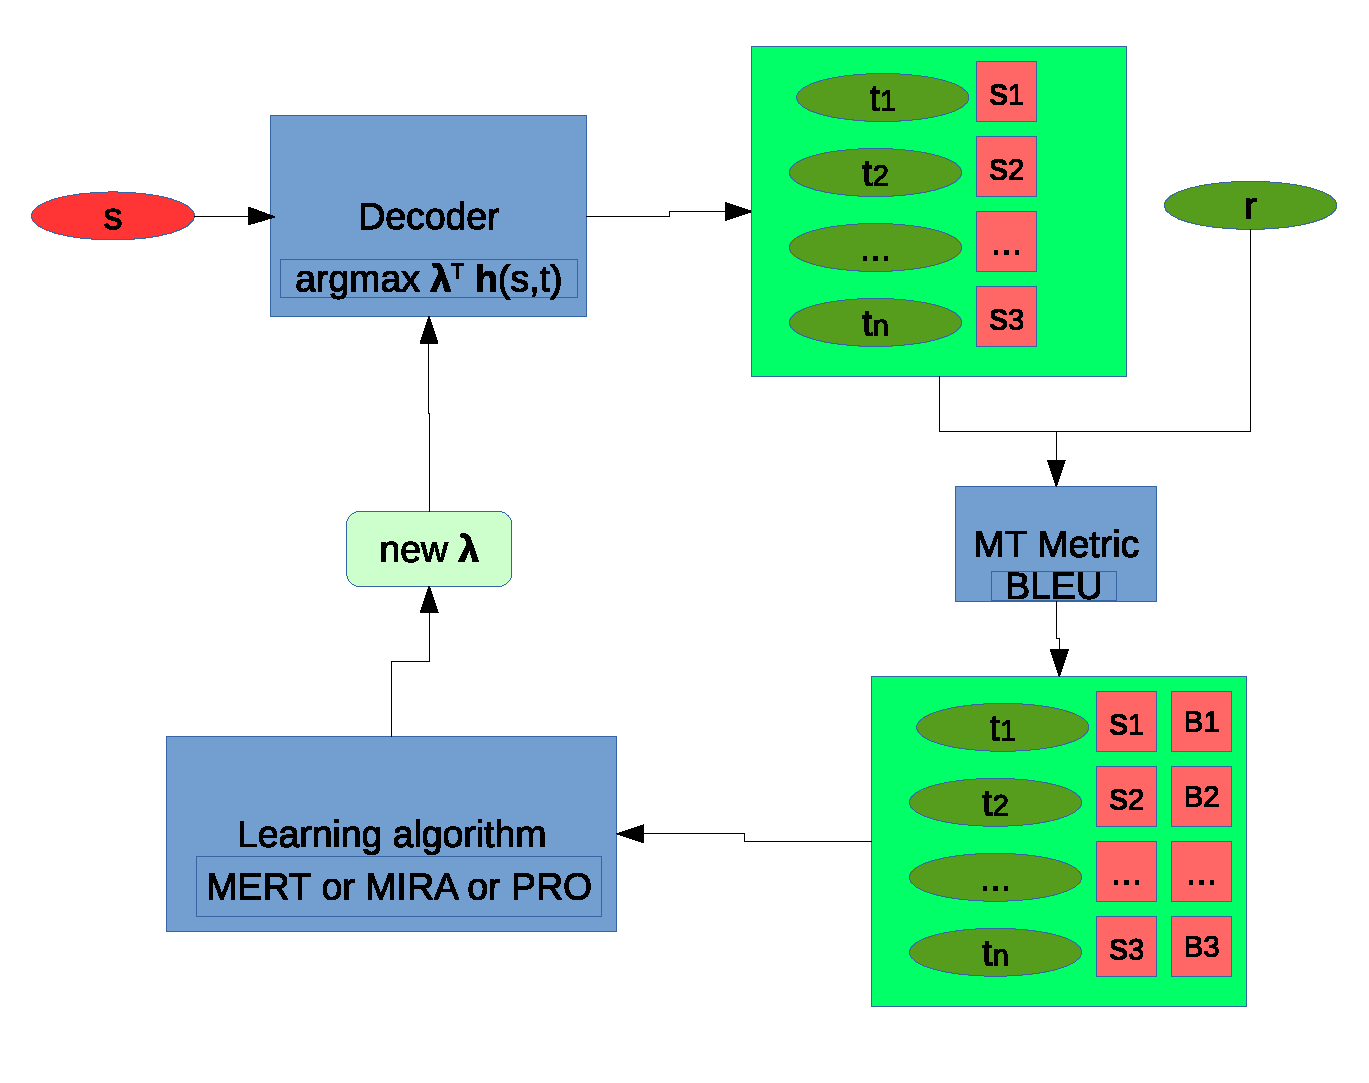
\includegraphics[width=0.70\linewidth]{drawing_discriminative_decoder_tuning5}}
\end{center}

}

\frame{\frametitle{MERT\cite{mert}}
\begin{itemize}
\item MERT is the most often used algorithm for this task
\item Optimizes parameters one by one
\item Directly optimizes objective
\item Works well with systems with small number of features
\end{itemize}
}

\frame{\frametitle{MERT\cite{mert}}
MERT optimizes only one parameter while keeping others fixed.
\begin{align}
\onslide<1->{score(s,t) & = \mathbf{\lambda}^T \mathbf{h}(s,t) \nonumber \\
                        & = \sum_i \lambda_i h_i(s,t)} \nonumber \\
\onslide<2->{& = \lambda_c h_c(s,t) + \sum_{i \neq c}\lambda_i h_i(s,t)} \nonumber \\
\onslide<3->{& = \lambda_c h_c(s,t) + u_c(s,t)} \nonumber
\end{align}

\onslide<4->{\begin{center}
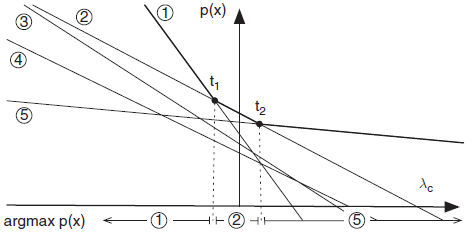
\includegraphics[width=0.60\linewidth]{MERT}
\end{center}}

}

\frame{\frametitle{MERT\cite{mert}}
\begin{center}
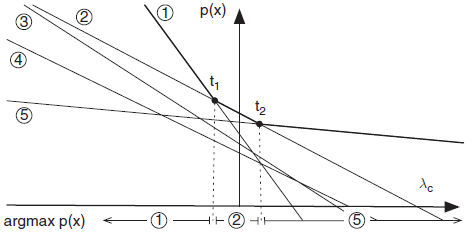
\includegraphics[width=0.60\linewidth]{MERT}
\end{center}

\begin{itemize}
\item Extract all \textbf{threshold points} where argmax changes
\pause \item Evaluate each set of threshold points with BLEU score
\pause \item Take the best one and then go again trough the decoding loop
\end{itemize}
}


\frame{\frametitle{MERT\cite{mert}}
\begin{center}
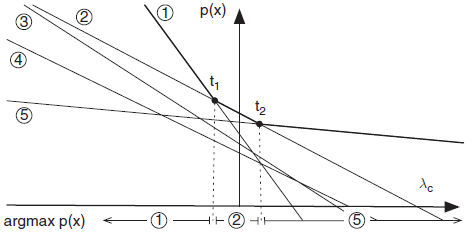
\includegraphics[width=0.60\linewidth]{MERT}
\end{center}

\begin{align}
\onslide<1->{score(s, t_1) & = score(s, t_2) \nonumber}
\onslide<2->{\\ \lambda_c h_c(s,t_1) + u_c(s,t_1) & = \lambda_c h_c(s,t_2) + u_c(s,t_2) \nonumber \\ \nonumber \\ \nonumber}
\end{align}

}

\frame{\frametitle{MERT\cite{mert}}
\begin{center}
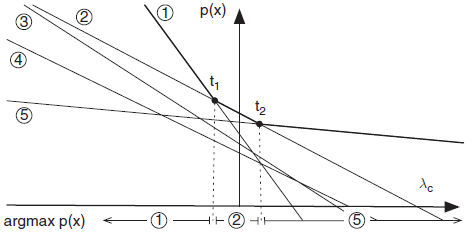
\includegraphics[width=0.60\linewidth]{MERT}
\end{center}

\begin{align}
score(s, t_1) & = score(s, t_2) \nonumber \\
\lambda_c \highlight{h_c(s,t_1)} + \highlight{u_c(s,t_1)} & = \lambda_c \highlight{h_c(s,t_2)} + \highlight{u_c(s,t_2)} \nonumber \\
\lambda_c &= \frac{u_c(s,t_1)-u_c(s,t_2)}{h_c(s,t_2)-h_c(s,t_1)} \nonumber
\end{align}

}

\frame{\frametitle{MERT\cite{mert}}
\begin{center}
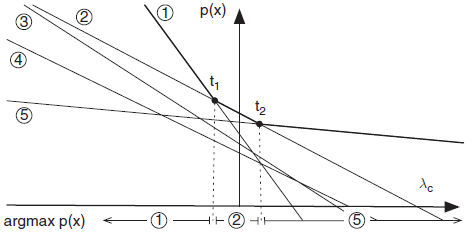
\includegraphics[width=0.60\linewidth]{MERT}
\end{center}

Few more tricks:
\begin{itemize}
\item We can speed up this by looking for top threshold points\\
start with the steepest line (smallest $h_c(s,t_1)$)\\
$score(x)=\lambda_c \highlight{h_c(s,t_1)} + u_c(s,t_1)$ \\
and find the most negative threshold point for that line
\pause \item Accumulate n-best lists over different decoder runs
\pause \item Average the weights of 3 MERT runs
\end{itemize}
}

\frame{\frametitle{MERT -- good and bad sides}
Good sides:
\begin{itemize}
\item Optimizes corpus level metrics directly.
\end{itemize}

Bad sides:
\begin{itemize}
\item Gets stuck in local minima\\example of finding the highest point in San Francisco \cite{smt_book}
\item Instable: BLEU varies a lot\\
requires at least 3 runs to make it significant \cite{multeval}
\item Cannot handle more than a dozen of features
\end{itemize}
}




\frame{\frametitle{PRO\cite{pro}}

PRO is a simple alternative that can allow training lots of features.

\pause First sample from n-best list many hypotheses pairs\\
$(t_{better}, t_{worse})$ where $eval(t_{better},r) > eval(t_{worse},r)$

\pause For each pair

\begin{align}
\visible<3->{score(s,t_{better}) & > score(s,t_{worse}) \nonumber }
\visible<4->{\\ \mathbf{\lambda}^T \mathbf{h}(s,t_{better}) & > \mathbf{\lambda}^T \mathbf{h}(s,t_{worse})  \nonumber}
\visible<5->{ \\ \mathbf{\lambda}^T (\mathbf{h}(s,t_{better})-\mathbf{h}(s,t_{worse})) & > 0 \nonumber}
\visible<6->{ \\ \mathbf{\lambda}^T (\mathbf{h}(s,t_{worse})-\mathbf{h}(s,t_{better})) & < 0 \nonumber}
\end{align}

\vspace{55pt}

}



\frame{\frametitle{PRO\cite{pro}}

PRO is a simple alternative that can allow training lots of features.

First sample from n-best list many hypotheses pairs\\
$(t_{better}, t_{worse})$ where $eval(t_{better},r) > eval(t_{worse},r)$

For each pair


\begin{align}
score(s,t_{better}) & > score(s,t_{worse}) \nonumber \\
\mathbf{\lambda}^T \mathbf{h}(s,t_{better}) & > \mathbf{\lambda}^T \mathbf{h}(s,t_{worse})  \nonumber \\
\mathbf{\lambda}^T (\highlight{\mathbf{h}(s,t_{better})-\mathbf{h}(s,t_{worse})}) & > 0 \nonumber \\
\mathbf{\lambda}^T (\highlight{\mathbf{h}(s,t_{worse})-\mathbf{h}(s,t_{better})}) & < 0 \nonumber
\end{align}

Train linear classifier with these as positive and negative training instance.

\onslide<2->{Repeat this many times until convergence in n-best list}

\onslide<3->{Repeat this with the loop trough the decoder}
}



\frame{\frametitle{MIRA}

\begin{itemize}
\item MIRA is a \textbf{large-margin} online learning algorithm similar to perceptron \cite{watanabe}.
\item Large margin is enforced between between hope and fear translations \cite{chiang2008online}
\begin{align}
t_{hope}= \argmax{t} score(s,t)+eval(t,r) \nonumber \\
t_{fear}= \argmax{t} score(s,t)-eval(t,r) \nonumber 
\end{align}
\item Batch version \cite{kbmira} present in Moses.
\end{itemize}


}

\frame{\frametitle{MIRA}

\begin{align}
t_{hope}= \argmax{t} score(s,t)+eval(t,r) \nonumber \\
t_{fear}= \argmax{t} score(s,t)-eval(t,r) \nonumber
\onslide<2->{\\ margin = score(s, t_{fear}) - score(s, t_{hope})  \nonumber}
\onslide<3->{\\ cost = BLEU(t_{hope}, r) - BLEU(t_{fear}, r) \nonumber}
\onslide<4->{\\ \mathbf{\lambda} \leftarrow \mathbf{\lambda}+\delta(\mathbf{h}(s,t_{hope})-\mathbf{h}(s,t_{fear})) \nonumber}
\onslide<5->{\\ \delta = min\left(C, \frac{margin+cost}{||h(s,t_{hope})-h(s,t_{fear})||^2}\right) \nonumber}
\end{align}

\onslide<5->{$\delta$ changes (unlike in Perceptron) to increase the margin}

\onslide<6->{Repeat this many times until convergence in n-best list}

\onslide<7->{Repeat this with the loop trough the decoder}


}


\frame{\frametitle{Lots of open problems}
	\begin{itemize}
		\item Evaluation metrics related:
		\begin{itemize}
		\pause	\item MIRA, PRO and Perceptron require sentence level metric (BLEU doesn't work well)
		\pause	\item use good metrics
		\pause	\item but good metrics oftend are not good for tuning
		\end{itemize}
		\pause\item Representation of space of translations:
		\begin{itemize}
		\pause	\item n-best list is too small (compared to exponential space)
		\pause	\item lattice and hyper-graph are better options but too complicated to use because metrics don't decompose to (hyper-)arcs
		\pause	\item n-best is not \textit{really} n-best because of pruning which breaks convergence guarantees \cite{violation}
		\end{itemize}
		\pause \item Optimization itself:
		\pause\begin{itemize}
		\pause	\item increase margin? minimize risk?
		\pause	\item latent variables (towards which derivation to optimize?)
		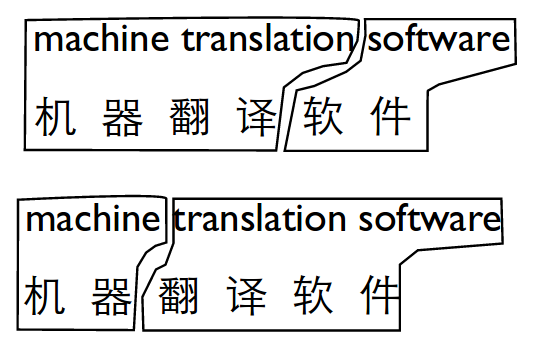
\includegraphics[width=0.30\linewidth]{MultipleDerivations}
		\end{itemize}
	\end{itemize}

}




%%%%%%%%%%%%%%%%%%%%%%%%%%%%%%%%%%%%%%%%%%%%%%%%%%%%%%%%%%%%%%%%%%%

\newcommand{\XXX}[1]{\textcolor{red}{#1}}
\newcommand{\system}[1]{\textsc{#1}}

\frame{\frametitle{Tuning task}

\begin{itemize}
\item So many things to choose in tuning (metric, algorithm, data, features...)
\pause \item Final performance usually measured by BLEU and not humans
\pause \item Organised Tuning Task on WMT15 to explore these options in proper way
\end{itemize}
}

\frame{\frametitle{Tuning task - system for tuning}

\begin{itemize}
\item Hiero Moses trained both for English-Czech and Czech-English on small dataset
\pause \item constrained version allowed 2000 sentence pairs for tuning
\pause \item constrained version allowed only dense features
\pause \item any tuning algorithm or metric tuning was allowed (even manually setting weights)
\end{itemize}
}

% \frame{\frametitle{Data}
%     \begin{table}[t]
%     \centering
%     \tiny
%     \begin{tabular}{llcc|cc|cc}
%     %           & Source & \begin{tabular}[c]{@{}l@{}}en-cs\\ \#sents\end{tabular} & \begin{tabular}[c]{@{}l@{}}cs-en \\ \#sents\end{tabular} & Tokens \\
%     		   &        & \multicolumn{2}{c|}{Sentences} & \multicolumn{2}{c|}{Tokens} & \multicolumn{2}{c}{Types} \\
%     		   & Source & cs & en & cs & en & cs & en \\
%     \hline
%     LM corpora &  News Commentary v8      &  162309  & 247966    &  3.6M & 6.2M & 162K & 81K  \\
%     TM corpora &  Europarl v7, CCrawl and News Comm. v9 &  \multicolumn{2}{c|}{911952} & 17.7M & 20.8M & 652K & 361K \\
%     Dev set &  newstest2014 &  \multicolumn{2}{c|}{3003}    & 51K & 60K & 19K & 13K        \\
%     Test set &  newstest2015 &  \multicolumn{2}{c|}{2656}   & 39K & 47K & 16K & 11K      \\
%     \end{tabular}
%     \caption{Data used in the WMT15 tuning task.}
%     \label{table:data}
%     \end{table}
% } 

% \frame{\frametitle{OOV words}
%     \begin{table}[t]
%     \centering
%     \small
%     \begin{tabular}{crr|rr}
%      & \multicolumn{2}{c|}{Dev} & \multicolumn{2}{c}{Test} \\
%     Direction & Token & Type & Token & Type \\ \hline
%     en-cs & 2570 & 2032 & 2003 & 1655 \\
%     cs-en & 3891 & 3415 & 3381 & 3011 \\
%     \end{tabular}
%     \caption{Out of vocabulary word counts}
%     \label{table:oov}
%     \end{table}
% }

\frame{\frametitle{Czech-English results}
    
\begin{table}
\begin{center}
\small
\begin{tabular}{rrr|r}
\textbf{System Name}   & \multicolumn{2}{c|}{\textbf{TrueSkill Score}} & \textbf{BLEU}\\
                       & \llap{Tun}ing-Only & All & \\
\hline
% \system{bleu-MIRA-dense	} & 0.3869 \\ \hline
% \system{AFRL		        } & 0.3824 \\ \hline
% \system{ILLC-UvA		} & 0.3740 \\ \hline
% \system{USAAR-Tuna	} & 0.3699 \\ \hline
% \system{bleu-MERT-dense		} & 0.3654 \\ \hline
% \system{DCU		        } & 0.3600 \\ \hline
% \system{METEOR-CMU		} & 0.3304 \\ \hline
% \system{bleu-MIRA-sparse	} & 0.3198 \\ \hline
% \system{HKUST			} & 0.3113 \\ \hline

\system{bleu-MIRA-dense		} & 0.153   & -0.182 & 12.28 \\
\system{ILLC-UvA		} & 0.108       & -0.189 & 12.05 \\
\system{bleu-MERT-dense		} & 0.087   & -0.196 & 12.11 \\
\system{AFRL		        } & 0.070   & -0.210 & 12.20 \\
% cluster border in tuning-only
\cline{2-2}
\system{USAAR-Tuna	} & 0.011       & -0.220 & 12.16 \\
\cline{3-3} % cluster border in all
\system{DCU		        } & -0.027  & -0.263 & 11.44 \\
% cluster border                           & \\
\cline{2-2} % \specialrule{.3em}{.2em}{.2em}
\system{METEOR-CMU		} & -0.101     & -0.297 & 10.88 \\
\system{bleu-MIRA-sparse	} & -0.150 & -0.320 & 10.84 \\
\system{HKUST			} & -0.150     & -0.320 & 10.99 \\ 
\hline
% \cline{1-2} % \specialrule{.3em}{.2em}{.2em}
\system{HKUST-LATE		} & --- & --- & 12.20 \\
\end{tabular}
\caption{Results on Czech-English tuning}
\label{table:results-csen}
\end{center}
\end{table}

} 

\frame{\frametitle{English-Czech results}
    
\begin{table}
%\begin{center}
\small
\hspace{-5mm}
\begin{tabular}{rrr|r}
\textbf{System Name}   & \multicolumn{2}{c|}{\textbf{TrueSkill Score}} & \textbf{BLEU}\\
                       & \llap{Tun}ing-Only & All & \\
\hline

\system{DCU			} & 0.320  & -0.342 & 4.96 \\
\system{bleu-MIRA-dense		} & 0.303  & -0.346 & 5.31 \\
\system{AFRL			} & 0.303  & -0.342 & 5.34 \\
\cline{2-3} % \specialrule{.3em}{.2em}{.2em}
\system{USAAR-Tuna	} & 0.214  & -0.373 & 5.26 \\
\cline{2-3} % \specialrule{.3em}{.2em}{.2em}
\system{bleu-MERT-dense		} & 0.123  & -0.406 & 5.24 \\
\cline{2-3} % \specialrule{.3em}{.2em}{.2em}
\system{METEOR-CMU		} & -0.271 & -0.563 & 4.37 \\
\cline{2-3} % \specialrule{.3em}{.2em}{.2em}
\system{bleu-MIRA-sparse	} & -0.992 & -0.808 & 3.79 \\ \hline
\system{USAAR-baseline-mira	} & ---   & ---  & 5.31 \\
\system{USAAR-baseline-mert	} & ---  & ---   & 5.25 \\


% \system{DCU			} & 0.3198 \\ \hline	
% \system{AFRL			} & 0.3151 \\ \hline			
% \system{bleu-MIRA-dense		} & 0.3071 \\ \hline
% \system{USAAR-Tuna	} & 0.2833 \\ \hline	
% \system{bleu-MERT-dense		} & 0.2659 \\ \hline
% \system{METEOR-CMU		} & 0.2544 \\ \hline
% \system{bleu-MIRA-sparse	} & 0.1767 \\ \hline
\end{tabular}
\caption{Results on English-Czech tuning}
\label{table:results-encs}
%\end{center}
\end{table}

} 

\frame{\frametitle{Word Penalty weights for English-Czech}
    %\begin{figure}[t]
    \begin{center}
    {
    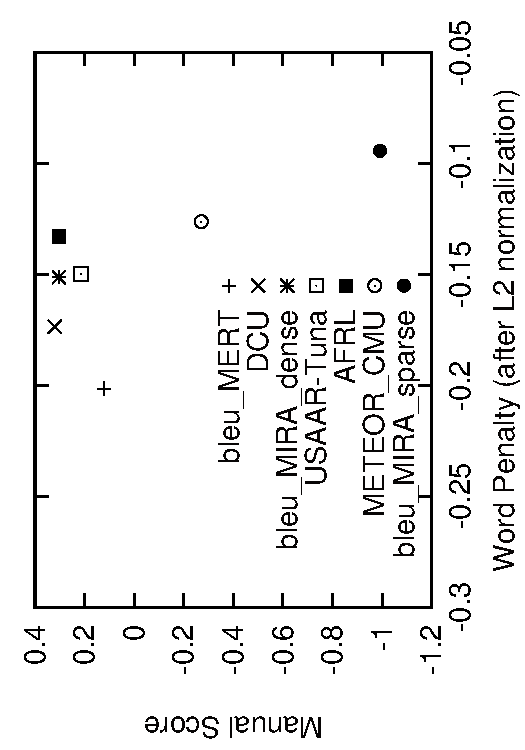
\includegraphics[width=0.6\columnwidth,angle=270]{wpplotL2.pdf}
    }
    \end{center}
    % \caption{Relation between the word penalty and the final performance of systems
    % translating from English to Czech.}
    % \label{wpplot}
    % \end{figure}
    \begin{itemize}
	\item Difficult to analyse individual weights but if we have to...
	\item All non-sparse systems find similar weights for WP
    \end{itemize}
} 

\frame{\frametitle{English-Czech PCA}
%        \begin{tabular}{cc}
    %\begin{figure}[t]
    \begin{center}
    %\vspace{-7mm}
    {
    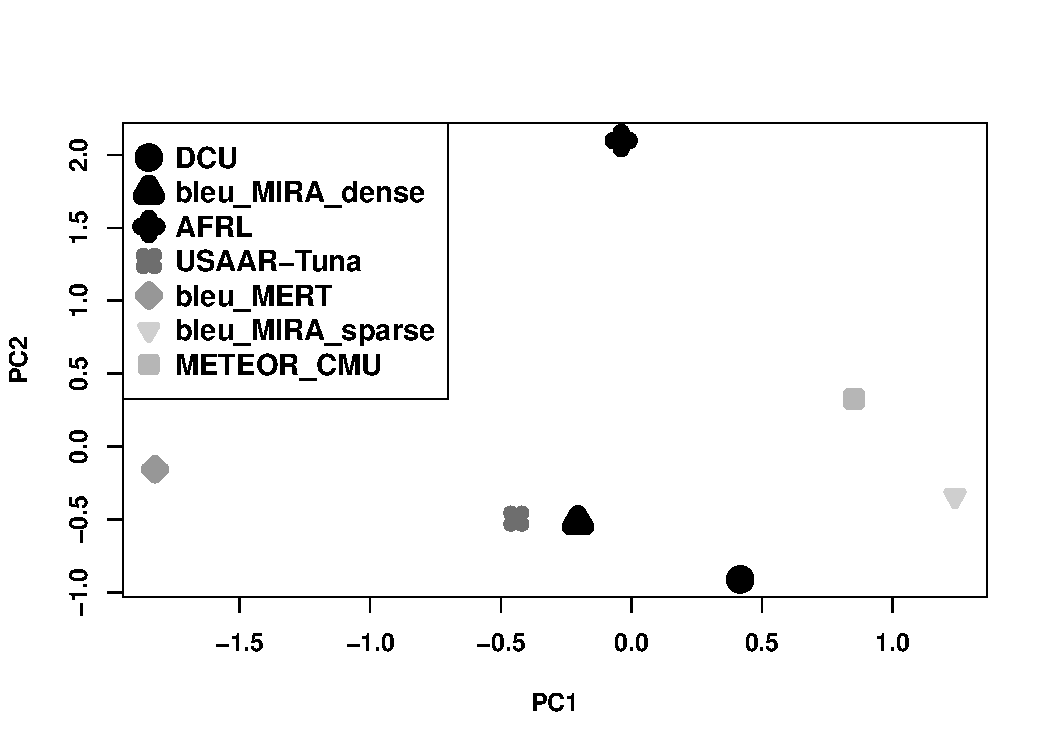
\includegraphics[width=0.99\columnwidth]{en-cs_PCA.pdf}
    }
    \end{center}
    %\caption{PCA for English-Czech. The darker the point, the higher the manual
    %score.}
    %\label{pca_encs}
    %\end{figure}
%	&
%    \begin{table}
%      \small
%      \begin{center}
%        \begin{tabular}{l|r|r}
%    
%                         &   PC1 &   PC2 \\\hline
%    LM0                  & \textbf{-0.69} &  0.44 \\
%    PhrasePenalty0       &  0.15 & \textbf{-0.63} \\
%    TranslationModel0\_0 & \textbf{-0.91} & -0.13 \\
%    TranslationModel0\_1 & \textbf{ 0.91} & -0.03 \\
%    TranslationModel0\_2 & -0.55 &  \textbf{0.72} \\
%    TranslationModel0\_3 &  0.36 &  \textbf{0.75} \\
%    TranslationModel1    &  0.42 &  \textbf{0.84} \\
%    WordPenalty0         & \textbf{ 0.84} &  0.27 \\
%        \end{tabular}
%    \caption{Loadings (correlations) of each component with each feature function for English-Czech}
%    \label{pca_loadings}
%      \end{center}
%    \end{table}
%\\ \end{tabular}
}

\frame{\frametitle{Table of contents}
    \begin{table}
      \small
      \begin{center}
        \begin{tabular}{l|r|r}
    
                         &   PC1 &   PC2 \\\hline
    LM0                  & \textbf{-0.69} &  0.44 \\
    PhrasePenalty0       &  0.15 & \textbf{-0.63} \\
    TranslationModel0\_0 & \textbf{-0.91} & -0.13 \\
    TranslationModel0\_1 & \textbf{ 0.91} & -0.03 \\
    TranslationModel0\_2 & -0.55 &  \textbf{0.72} \\
    TranslationModel0\_3 &  0.36 &  \textbf{0.75} \\
    TranslationModel1    &  0.42 &  \textbf{0.84} \\
    WordPenalty0         & \textbf{ 0.84} &  0.27 \\
        \end{tabular}
    \caption{Loadings (correlations) of each component with each feature function for English-Czech}
    \label{pca_loadings}
      \end{center}
    \end{table}
}

\frame{\frametitle{Czech-English PCA}
    
    %\begin{figure}[t]
    \begin{center}
    \vspace{-7mm}
    {
    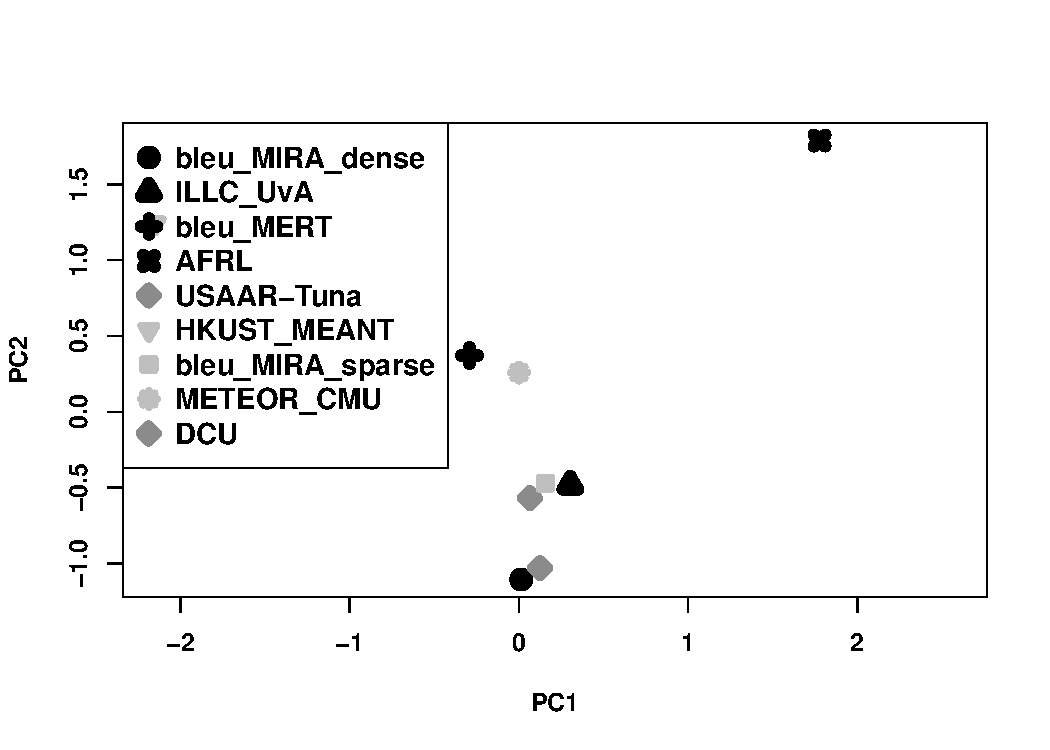
\includegraphics[width=0.90\columnwidth]{cs-en_PCA.pdf}
    }
    \end{center}
    %\caption{PCA for Czech-English. The darker the point, the higher the manual
    %score.}
    %\label{pca_csen}
    %\end{figure}
	\begin{itemize}
		\item No obvious pattern
		\item Very similar systems perform complitely differently
		\item Very different systems perform similarly
	\end{itemize}

} 


\section{Conclusion}


\frame{\frametitle{Conclusion}
	\begin{itemize}
		\item Tuning is a \textbf{standard procedure} of most modern MT systems
		\pause \item But still \textbf{difficult} in many respects
		\pause \item \textbf{Tuning Task} will happen on again WMT16
		\pause \item Questions?
	\end{itemize}

}




%

\frame{\frametitle{Violated Perceptron and Early update}
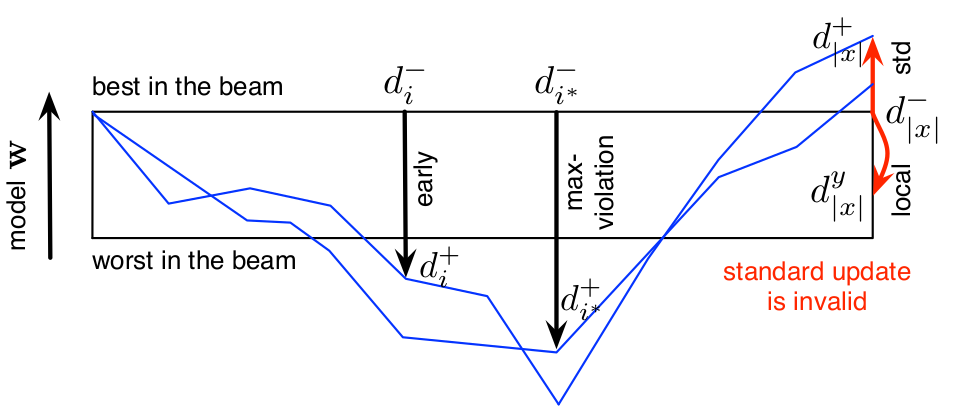
\includegraphics[width=0.90\linewidth]{ViolatedPerceptron}

\begin{itemize}
\item Early update \cite{earlyUpdate} whenever gold hypothesis falls out of beam (smallest violation appears)
\item Max-violation update \cite{violation} when violation (error) is highest
\item Doesn't exist in Moses nor Joshua (but maybe after MT Marathon?)
\end{itemize}

}


\section{Bibliography}
\begin{frame}[allowframebreaks]
\tiny
\frametitle{Bibliography}
\bibliographystyle{apalike}
\bibliography{BIB}
\end{frame}

\end{document}

